\documentclass[a4paper]{article}

%%% packages %%%%%%%%%%%%%%%%%%%%%%%%%%%%%%%%%%%%%%%%%%%%%%%%%%%%%%%%%%%%%%%%%
\usepackage{graphicx}
\usepackage{amsmath,amssymb}
\usepackage{alltt}
\usepackage{natbib} % please use \citep and \citet instead of \cite

\usepackage{hyperref}
\usepackage{xcolor}
\definecolor{dark-red}{rgb}{0.4,0.15,0.15}
\definecolor{dark-blue}{rgb}{0.15,0.15,0.8}
\definecolor{medium-blue}{rgb}{0,0,0.5}
\hypersetup{
	colorlinks, linkcolor={dark-red},
	citecolor={dark-blue}, urlcolor={medium-blue}
}

\graphicspath{{./figs/}}
\DeclareGraphicsExtensions{.pdf}

\setlength{\parindent}{0mm}

\usepackage{fancyhdr}

%%% %%%%%%%%%%%%%%%%%%%%%%%%%%%%%%%%%%%%%%%%%%%%%%%%%%%%%%%%%%%%%%%%%%%%%%%%%

\makeatletter
\newcommand{\seminar}{Seminar Cyber-Physical Systems (WS 2019/20)}
\title{\textbf{Prioritized Sweeping Neural DynaQ:\\ Boost Learning by Dreaming}}\let\Title\@title
\newcommand{\sTitle}{Prioritized Sweeping Neural DynaQ}
\newcommand{\AuthorName}{Alexander Osiik}
\author{\AuthorName\\
	\href{mailto:alexander.osiik@student.uni-luebeck.de}{alexander.osiik@student.uni-luebeck.de}\\
	\small \seminar\\
%	\small Service Robotics Group\\
	\small Institute of Computer Engineering, University of L\"ubeck\\
}\let\Author\@author
\makeatother

\pagestyle{fancy}
\renewcommand{\footrulewidth}{0.4pt}
\lfoot{\seminar}
\cfoot{}
\rfoot{\thepage}
\lhead{\AuthorName}
\rhead{\sTitle}

%%% %%%%%%%%%%%%%%%%%%%%%%%%%%%%%%%%%%%%%%%%%%%%%%%%%%%%%%%%%%%%%%%%%%%%%%%%%

\begin{document}
	\maketitle
	
	\begin{abstract}
		\noindent%
		Hier beschreiben welche Hintergründe und Analogien aus der Biologie Reinforcement Learning hat.\\
		State of the Art.\\
		Was Zielsetzung im Original-Paper war, wie sie erreicht wurde und wie es im Projekt umgesetzt wurde.
	\end{abstract}
	
	
	\section{Introduction}
	\label{sec:introduction}
%	Swarm robotics~\citep{brambilla13} bla bla bla.
%	\citet{hamann18} describes bla bla bla
%	see Sec.~\ref{sec:results}
\par The hippocampus is the main memory of our brain and the switch point between short-term and long-term memory. \citet{OKEEFE1971171} observed in several rat experiments that if there is a disturbance in this area, no new information can be stored in the brain. Regarding animals, the hippocampus is known to be important for navigation since the discovery of place cells, which signal the current allocentric location of the animal in the environment \citep{Maguire}. Interaction within the environment leads to activation these place cells. They are engaged during the consolidation of spatial memories. However, it has been observed that these activations also occur during rest or sleep, at a significally faster pace. This reactivation can be seen as a reprocessing of the experience gained during the day, something that is usually the case when dreaming \citep{HippocampalReplaysGirard}.

\par \citet{NeuralDynaQ} presented an approach to convert the reactivation of the hippocamus' place cells into a reinforcement learning model.  \cite{OKEEFE1971171} postulated that the hippocampus functions as a spatial map, where single hippocampal neurons increased their firing rate whenever a rat traversed a particular region of an environment, as concluded by \cite{Nakazawa}.
		
\subsection{Experimental setup}
\par \cite{NeuralDynaQ} set up a experimental task, which was derived and slightly modified from \cite{GUPTA2010695}. The environment consisted of two succesive T-mazes with lateral return corridors and rewarding food pellets on each side, see Figure \ref{fig:setup}. A rat was placed in the maze, and trained to make a decision at position T2, with the objective of getting the reward on the left or right hand side based on the task pursued at the moment. The tasks were 1) always turn right, 2) always turn left, 3) alternate between left and right. At reward locations, the rat's hippocampal replays were analyzed. It has been shown that the rats reflected recently experienced trajectories, and, in addition, also those that occurred a longer time ago.
		
\begin{figure}[t]
	\centering
	\includegraphics[angle=0,width=0.5\textwidth]{./figs/setup.png}
	\caption{\label{fig:setup}Discretized experimental setup. The agent has to make a decision at points T1 and T2, in which the dicision at T2 leads to one of the rewarding sites. \citep{NeuralDynaQ}}
\end{figure}
		
\par To mathematiacally model and explain the hippocampal replay phenomenon, algorithms from the Dyna family of algorithms were used. Dyna is an integrated architecture for learning, planning and reacting, proposed by \cite{Dyna}, see Figure~\ref{fig:dyna}. The Dyna idea is a trivial approach that planning is equivalent to trying out multiple things in the own mind, under the condition that a certain internal model of the problem exists. Ultimately, this architecture was chosen because it is designed to make the best possible use of alternation between on-line and off-line learning phases \citep{Dyna}. \cite{NeuralDynaQ} concentrated on the Q-learning version of Dyna (Dyna-Q) extended by prioritized sweeping, by that optimizing the choice of reactivated cells.


	\begin{figure}[h]
		\centering
		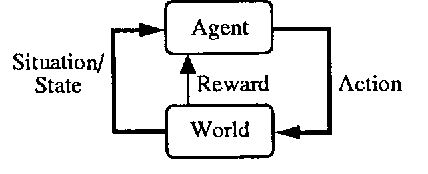
\includegraphics[angle=0,width=0.7\textwidth]{./figs/Dyna-Figure1.png}
		\caption{\label{fig:dyna}The Problem Formulation Used in Dyna. The agent's objective is to maximize the total reward it receives over time. \citep{Dyna}}
	\end{figure}
\section{Reinforcement Learning}
To further understand the underlying methods it is important to know the general mathematical rules and machine learning approaches. In the following, the terminology aswell as mathematical background of the research subject is briefly summarized and explained. 
%	\label{sec:rl}
%	see Fig.~\ref{fig:image}	

\subsection{Markov Decision Problem}
	A Markov Decision Problem (MDP) is a model for problems, where an agent tries to interact with the environment in such way that the utmost reward is achieved. Specifically, the robot is moving (\textit{transition}) through various \textit{states}, having chosen a specific \textit{action} in each state. Each \textit{reward} is determined by initial state, the action and the following state. 
	All transitions are not deterministic, but rather probabilistic, where each probability only depends on the current state and the current action. This memoryless property of stochastic processes is refered to as \textbf{Markov condition}. That way there has to be one initial state, but multiple end states are possible.\\
	The main goal is to find a reward maximizing \textbf{policy}, by which the agent selects actions where the maximum reward can be expected. This policy is an optimal plan, or sequence of actions, from start to a goal \citep{Lecture}.
	\par A markov decision process consists of
	\begin{itemize}
		\item Set of states $S:$ $\{s_1,s_2,\dots, s_n\}$
		\item Set of actions $A:$  $\{a_1,a_2,\dots, a_n\}$ 
		\item Transition function, which is the probability of going from state $s$ to state $s'$ via action $a$: $T: S\times A \times S$
		\item  Reward function $R: S\times A \times S \rightarrow \mathbb{R}$
	\end{itemize}
	The main goal is to find an optimal policy $\Pi$ and exploration factor $\gamma$, where
	\begin{itemize}
		\item $\Pi$ is the policy, where an optimal action is assigned to each state
		\item $\gamma \in [0,1]$ is the discount factor. This factor determines the degree of exploration for the agent. For $\gamma=0$, the agent will stick to the policy, and explot the current (possibly) optimal policy. For $\gamma=1$, the agent will take into account the next states reward, leading to exploration behaviour. A value <1 is a contraint, which limits the maximal obtainable reward, leading to a reduction of cycles.
	\end{itemize}
	The \textbf{V-values} and \textbf{Q-values} are certain grading schemes used To solve MDPs. The values are the total reward the agent can expect if it performs the optimal, or maximally benefitting, action $a$ in state $s$, and continues to act optimally thereafter:
	\begin{equation}\label{eq:vvalue}
		V^*(s) = \max_{a \in A} \sum_{s' \in S}^{} T(s,a,s')[R(s,a,s')+\gamma V^*(s')]
	\end{equation}
	As the values from equation \ref{eq:vvalue} are hard do compute, a technique called \textbf{value iteration} is used. It is used do discretize the equation: 
	\begin{equation}\label{eq:value-iteration}
		V^*(s) = \max_{a \in A} \sum_{s' \in S}^{} T(s,a,s')[R(s,a,s')+\gamma V^*(s')]
	\end{equation}
	where $k$ is the radius from the goal state to the agent. For example, regarding the manhattan norm in a 2D plane, the amount of steps the agent has left until it reaches an end state.\\
	After that, \textbf{policy extraction} is performed. It is the assignment of an action to each state, maximizing the expected total reward:
	\begin{equation}
		\Pi^*(s) = \text{arg}\max_{a \in A} \sum_{s' \in S}^{} T(s,a,s')[R(s,a,s')+\gamma V^*(s')]
	\end{equation}
	\begin{figure}[t]
		\centering
		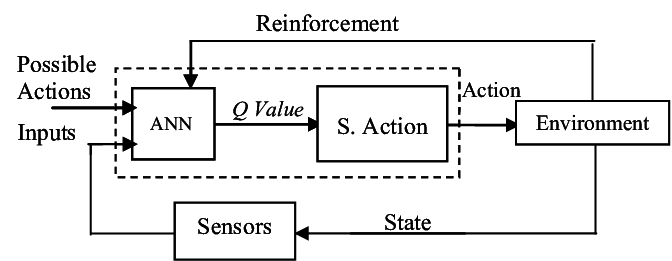
\includegraphics[angle=0,width=0.7\textwidth]{./figs/RL_ANN.png}
		\caption{\label{fig:qlearn}The structure of reinforcement learning based on an Artificial Neural Network \citep{HatemRL}}
	\end{figure}
\subsection{Q-Learning}
Q-Learning is a model-free reinforcement learning algorithm which converges to optimal policy even if if the performed actions are suboptimal \citep{Lecture}. The letter \textbf{Q} stands for \textbf{quality} of a certain action in a given state, as the values represent the maximum discounted future reward when action $a$ in state $s$ is performed. Q-values are calculated similar to the value iteration in Equation \ref{eq:value-iteration}:
	\begin{equation}\label{eq:qlearn}
Q^*(s,a) = \max_{a \in A} \sum_{s' \in S}^{} T(s,a,s')[R(s,a,s')+\gamma V^*(s')]
\end{equation}
The funcion $Q(s,a)$ can be estimated using Q-Learning, which is a form of \textbf{Temporal Difference Learning} (TD). TD means that the performs an update after every action based on a maximum reward estimate, and not only after receiving the reward.
\par  Here, value $Q(s,a)$ is iteratively updated using the \textbf{Bellman Equation}: \\\\
	\begin{equation}\label{eq:qupdate}
Q(s,a) \leftarrow Q(s,a) + \alpha [r + \gamma \max_{a' \in A}Q(s',a')-Q(s,a)]
\end{equation}
The Q-values are represented in a \textbf{Q-table} where each cell represents the highest achievable reward performing the state-action pair $(s\in S, a\in A)$. This makes Q-learning suitable for small environments only, as an increase in states or actions increases the memory consumption quadratically. 
\par The challenge is to tune the parameters $\alpha , \gamma$ such that the best possible policy is found in minimal time.

	
	\section{GALMO}
	\label{sec:galmo}
	\textbf{TODO}
	\begin{itemize}
		\item Brief summary of the proposed algorithm (GALMO)
		\item Why this algorithm? What are the benefits of dynamic DQN over simple Q-Learn?
		\item Present results
	\end{itemize}
	
	
	\section{Project}
	\label{sec:project}
	As part of practical work, a simplified T-maze configuration with a discrete environment similar to the work of \cite{NeuralDynaQ} has been reproduced. The programming language of choice was Python, as it offers many up-to-date machine learning libraries and allows a readable and understandable implementation.
	\par For the successful completion of task 3 (reward sites alternate) the state space was extended by two components: the left side reward memory (L) and the right side reward memory (R). 
	As proposed by \citet{NeuralDynaQ}, they take a value 1 if the last reward was obtained on that side, 0.5 if the penultimate reward was obtained on that side and 0 if that side has not been reward during the last 2 runs. Thus Q-Learning is also applicable in situations that actually depend on the past, by this violating the Markov condition.\\
	\par \textbf{TODO}
	\begin{itemize}
		\item Umsetzung von Q-Learning in Python
		\item DQN
		\item Implementierung GALMO? prolly not, fam
	\end{itemize}
	
	
	\section{Results}
	\label{sec:results}
	\textbf{TODO}\\
	Compare own results and GALMO results
		
	
	
	\section{Conclusion}
	\label{sec:conclusion}
	\textbf{TODO}
	
	
	\footnotesize
	\bibliographystyle{plainnat}
	\bibliography{./main}
	
\end{document}
